\subsection{Elektrische Kapazität C \hfill $[F]$}
    \begin{minipage}{0.49\linewidth}
        \begin{center}
            Im Vakuum:
            \mathbox{C_0 = \frac{Q}{U} = \varepsilon_0 \frac{A}{l}}
        \end{center}
    \end{minipage}
    \begin{minipage}{0.49\linewidth}
        \begin{center}
            Materie (Dielektrikum mit $\varepsilon_m$):
            \begin{empheq}[box=\fbox]{align*}
                C_m &= \varepsilon_m C_0\\
                U_m &= \frac{U_0}{\varepsilon_m}
            \end{empheq}
        \end{center}
    \end{minipage}

    Beispiel Kugelkondensator:\\
    \begin{minipage}{0.49\linewidth}
        \begin{center}
            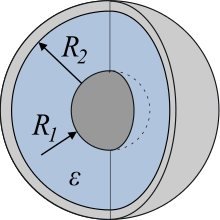
\includegraphics[width = 0.49\linewidth]{src/images/kugelkondensator.png}
        \end{center}
    \end{minipage}
    \begin{minipage}{0.49\linewidth}
        \begin{center}
            \begin{empheq}[box=\fbox]{align*}
                C &= 4 \pi \varepsilon \left(\frac{r_1 \cdot r_2}{r_2 - r_1}\right)
            \end{empheq}
        \end{center}
    \end{minipage}

    \begin{minipage}{0.49\linewidth}
        \begin{center}
            Ladestrom Kondensator:
            \begin{empheq}[box=\fbox]{align*}
                I(t) &= I_0 \cdot e^{\left(-\frac{t}{R \cdot C}\right)}\\
                I(0) &= I_0 = \frac{U}{R_{\text{tot}}}\\
                I(\infty) &= 0
            \end{empheq}
        \end{center}
    \end{minipage}
    \begin{minipage}{0.49\linewidth}
        \begin{center}
            Einschieben von Dielektrika in einen Plattenkondensator: Die Energieverteilung verändert sich bis ein Gleichgewichtszustand erreicht ist:
            \begin{empheq}[box=\fbox]{align*}
                0 &= dW_{\text{tot}}\\
                 &\scriptstyle= dW_{\text{Feld}} - dW_{\text{Batt}} + dW_{\text{Diel}}
            \end{empheq}
        \end{center}
    \end{minipage}